\section{Workflow Overview}

\begin{frame}{Introduction}
%\begin{itemize}[<+>]
\begin{itemize}
\item High-level principle:
\begin{itemize}
\item[-] data: many input/output example pairs.
\item[-] models \textbf{learn from examples}.
\end{itemize}
 \pause
\item For example:
\begin{itemize}
\item[-] You will \alertbf{not} write a hard-coded program which translates a English sentence to a French sentence.
 \pause
\item[-] Instead: you will \textbf{train} your \textbf{model/neural network} by letting it see many (many!) examples of paired English-French sentences (\textbf{training data}).
\end{itemize}
 \pause
\item Your model has \emphbf{parameters}, which are initially random.\\
\begin{itemize}
\item[-] \textbf{Training will modify/optimize the model parameters} such that they would minimize a \textbf{loss function} (correlated to the task you want to solve).
\end{itemize}
\pause
\item Your model and training setup have \emphbf{hyper-parameters}:
\begin{itemize}
\item[-] You train multiple models with different hyper-parameters and select the best model based on its \textbf{validation data} performance.
\end{itemize}
 \pause
\item The final model is evaluated on the \textbf{test data}.
%; in the example of translation, sentences unseen during the training.
\end{itemize}
\end{frame}

\begin{frame}{Typical Deep Learning Workflow\\ (supervised learning)}
\begin{itemize}
\item Define/obtain: \textbf{task, dataset}
\item Define \textbf{model}
\item Define \textbf{loss} and \textbf{optimization algorithm}
\item Do \textbf{training} and \textbf{hyper-parameter tuning}
\item Evaluate its performance using an \textbf{evaluation metric(s)}\\
(:= make prediction on the test data using the trained model; requires some search algorithm depending on the task)
\end{itemize}
\end{frame}

\begin{frame}{Task and Data}
Image classification? Speech recognition? Image question answering?\\
\vspace{5mm}
\textbf{For any problem,}
you should know your \textbf{\alert{task}} and \textbf{\alert{dataset}}:
\begin{itemize}
\item What are the \textbf{inputs \& outputs} to the system?
\item What are the \textbf{basic statistics} of the data?\\
 (size of the data, number of output classes, ...)
\item Which metric do you use to \textbf{evaluate} the final model performance?
\end{itemize}
\vspace{2mm}
General recommendation: take some time looking into data examples,
before building a model.
\end{frame}

\begin{frame}{Task and Data (cont'd)}
\textbf{Example 1:}
\vsp
\begin{itemize}
\item Task: \textbf{Image classification}
\pause
\item Nature of the problem: input = image, output = class label.
\pause
\item Dataset statistics? For example:
\begin{itemize}
\item[-] Number of training samples: 10K 100K? 1M? images (is this big? toy task?)
\item[-] Number of classes: 10? 100? 1000? classes (dog, cat, airplane,...)\\ (is this big? small/toy task?)\\
\end{itemize}
\pause
%Classifying between just dog and cat is different from classification among 1000 classes.
\item Evaluation metric: classification error or accuracy (number of correctly classified test images divided by the total number of test images).
\item Extra aspect: is this a standard benchmark dataset? do people publish on this dataset? What are the baseline models/performance? 
\end{itemize}
\end{frame}

\begin{frame}{Task and Data (cont'd)}
\textbf{Example 2:}
\vsp
\begin{itemize}
\item Task: \textbf{Machine Translation}
\pause
\item Nature of the problem:\\ input = text in the source language, output = text in the target language.\\
Each example: bilingual sentence pair.
\pause
\item Dataset statistics? For example: 
\begin{itemize}
\item Number of training sample:\\ 100\,M bilingual training sentence pairs (is this big? small/toy task?)
\item Vocabulary: word? sub-word? character? (choice for your system)
\item Vocabulary size: 30\,K in source and 40\,K tokens in target language.
\item (Domain of texts: News? European parlament?)
\end{itemize}
\item Evaluation measure: BLEU \citem{PapineniRWZ02}.
\end{itemize}
\end{frame}

\begin{frame}{Modeling}
\begin{itemize}
\item Architecture \& type of your model will depend on the task.\\
\item In particular: different input/output modalities.
\item \textbf{In Section 3}: different types of neural network architectures will be reviewed.
\item Here: quick reminder on basics of neural networks,\\
to introduce \textbf{key words} and practicalities.
\end{itemize}

\end{frame}

\begin{frame}{Modeling:\\Reminders on neural networks}
A Neural Network:
\begin{itemize}
\item is a \textbf{parameterized} function (whose parameters are \textit{learned} from data).\\
\pause
\item transforms a \textbf{vector to another vector} (the most standard case).\\
\pause
\item Such a layer can be composed multiple times (output of a layer becomes input to next layer...etc) to make the model \textbf{deeper}. \\Each layer with its own parameters (in principle).
\end{itemize}
\end{frame}


\begin{frame}{Modeling:\\Reminders on neural networks}
\textbf{Two basic operations.} Let $d_\text{in}$ and $d_\text{out}$ denote positive integers.

A typical \textbf{one-layer} feed-forward neural network transforms input $x\in\mathbb{R}^{d_\text{in}}$ to output $z\in\mathbb{R}^{d_\text{out}}$ as follows:
\begin{itemize}
\item \textbf{Affine transformation} (\emphbf{Linear layer}): $y = Wx + b$ where $W\in\mathbb{R}^{d_\text{out} \times d_\text{in}}$ is a \emphbf{weight matrix} and $b\in\mathbb{R}^{d_\text{out}}$ is a \emphbf{bias} vector.
$y\in\mathbb{R}^{d_\text{out}}$.\\
$W$ and $b$ are \emphbf{trainable parameters}.
% Loosely this is often refer to as a \textit{linear layer}.
\begin{figure}
\centering
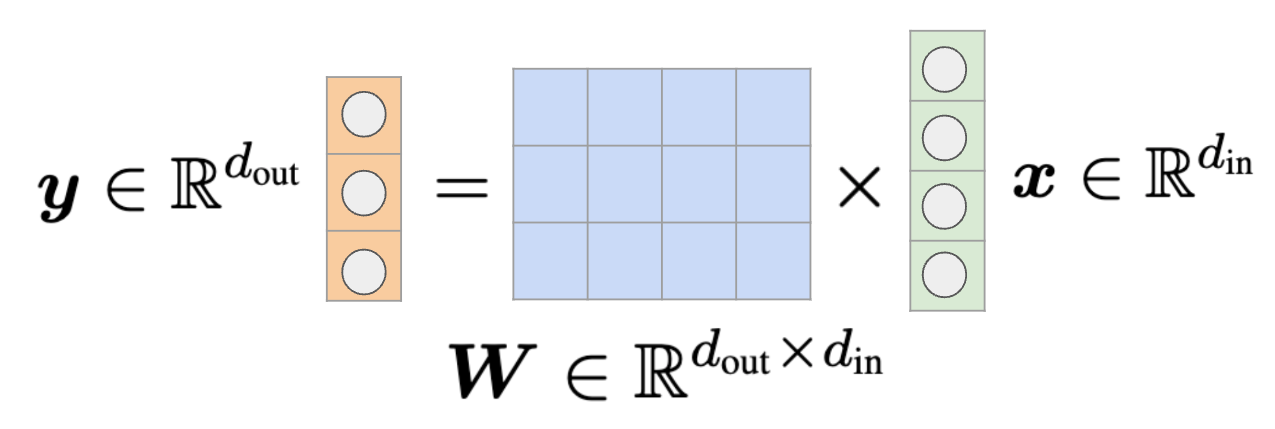
\includegraphics[width=0.80\linewidth]{./figures/linear.png}
\end{figure}
\pause
\item Element-wise non-linear \textbf{activation function}: $z = \sigma(y) \in\mathbb{R}^{d_\text{out}}$
\pause
\end{itemize}
We can compose many layers (an output of a layer becomes an input to the next layer...etc) to obtain a \emphbf{deep} neural net.
\end{frame}

\begin{frame}{Modeling:\\Reminders on neural networks (cont'd)}
\begin{minipage}{0.6\linewidth}
\textbf{Activation functions.}
\begin{itemize}
\item Commonly used functions:\\ \emphbf{sigmoid}, \emphbf{tanh},\\ rectifier linear unit (\emphbf{ReLU}).
\item More exotic functions:\\ ELU, GELU, SiLU...
\item For normalized output: \emphbf{softmax}.
\end{itemize}
\end{minipage}
\hspace{-8mm}
\begin{minipage}{0.38\linewidth}
\begin{figure}
                        \centering
                        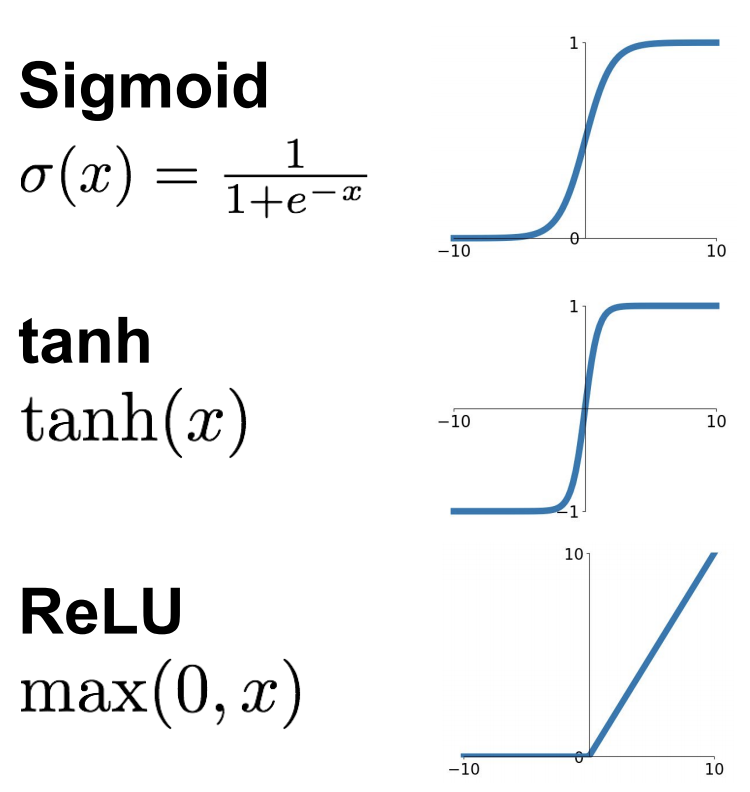
\includegraphics[width=0.95\linewidth]{./figures/activation.png}
\end{figure}
\tiny{Figure taken from \citem{stanford2019training}}
\end{minipage}
\end{frame}

\begin{frame}{Activation functions (cont'd)}
\textbf{Softmax function:}\\
\vsp
\begin{itemize}
\item[-] Let $d$ denote a positive integer
\item[-] Input $x\in\mathbb{R}^d$ is an arbitrary vector.
\item[-] Output $y\in\mathbb{R}^d$ defines a \emphbf{probability distribution}
\end{itemize}
% Input $x\in\mathbb{R}^n$, output $y\in\mathbb{R}^n$.\\
\vsp
For $1 \leq i \leq d$, $i$-th entry of vector $y\in\mathbb{R}^d$ is defined as: 
\[
 y_i = \displaystyle \dfrac{\exp(x_i)}{\displaystyle \sum_{n=1}^{d} \exp(x_n)}
\]
\vsp
The output vector $y$ has the following properties:
\begin{itemize}
\item All entries which are positive: For $1 \leq i \leq d$, $y_i > 0$.
\item The sum of all entries is one (normalized output): $\displaystyle \sum_{i=1}^{d} y_i = 1$.
\end{itemize}
The input $x$ to the softmax function is often called \emphbf{logit}.
\end{frame}

\begin{frame}{Model: illustration}
\begin{figure}
\centering
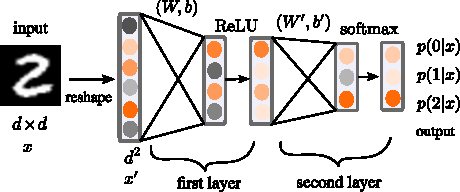
\includegraphics[width=0.90\linewidth]{./figures/nn_intro.pdf}
\end{figure}
\begin{itemize}
\item 2-layer feed-forward neural network model for\\
classification of $d$ by $d$ images of digits to 3 possible classes: 0, 1 or 2.
\end{itemize}
\end{frame}


% \begin{frame}{Modeling:\\Reminders (cont'd)}
% 
% Models have \emphbf{hyper-parameters} such as:
% \vsp
% \begin{itemize}
% \item Number of layers.
% \item Size of each hidden layer.
% \item ... other model specific hyper-parameters...
% \end{itemize}
% \vsp
% These hyper-parameters must be \emphbf{tuned}:
% \vsp
% \begin{itemize}
% \item Hyper-parameters are not \textit{learned} by the training algorithm!
% \item They are set before training and remain the same throughout training (with a few exceptions).
% \item Tuning: specify a set of hyper-parameters, train the model, and check its performance on some validation data, repeat until you obtain a "good" model.
% \item Tuning is a practice you learn from hands-on experience!
% \item We will come back to this in exercises.
% \end{itemize}
% \end{frame}

\begin{frame}{Training}
\textbf{Training}: optimization process to find the optimal values for the model parameters for the loss function.
\begin{itemize}
\item Before training: model parameters are random. 
\item After training: model parameters should have values which allow the model to solve the task!
\end{itemize}
\vsp
For that we must define:
\begin{itemize}
\item \textbf{Loss function}: function of model parameters to be minimized during training.
\item \textbf{Optimizer}:
specification of optimization algorithm with its hyper-parameters.
\end{itemize}
\vsp
\emphbf{Training hyper-parameters} need to be tuned: e.g. learning rate...
\end{frame}

\begin{frame}{Training: Loss}
\begin{itemize}
\item Let $N$ and $P$ denote positive integers.\\
A super script $i$ in $x^i$ denotes $i$-th training example.
\item \emphbf{Training data} $\{(x^1, y^1), ..., (x^N, y^N)\}$\\
is a set of $N$ input $x^i$ and output/target $y^i$ pairs.
\item[-] The exact specification of the nature of $x^i$ and $y^i$ does not matter here (you can assume that they are both vectors).
\pause
\item We want to train our \emphbf{model} $f_{\theta}$ with $P$ trainable \emphbf{parameters} $\theta \in \mathbb{R}^P$.
\item[-] \emphbf{Loss function} $\displaystyle \mathcal{L(\theta)} = \dfrac{1}{N} \sum_{i=1}^N \ell\left(f_{\theta}(x^i), y^i\right)$\\
with some function $\ell$ (dependent of the problem) which ``\textit{compares}'' each model output/prediction $f_{\theta}(x^i)$ and the target (true label) $y^i$.
% \item Typical notation: ``hat'' for the model prediction:  $\hat{y}^i = f_{\theta}(x^i)$
\end{itemize}
\end{frame}

\begin{frame}{Training: Loss (cont'd), Reminders}
\vspace{-5mm}
% Reminders:
% \vsp
For \textbf{regression} problems, let $d$ denote a positive integer (target vector size)
\begin{itemize}
\item Target $y^i  \in \mathbb{R}^d$ is a \textbf{vector}
\item so is the model output $f_{\theta}(x^i) \in \mathbb{R}^d$.\\
\vsp
\end{itemize}
Using the squared error
$\ell\left(f_{\theta}(x^i), y^i\right) = \|f_{\theta}(x^i) - y^i  \|^2_2$ we get the\\
\emphbf{Mean Squared Error (MSE) Loss}: $\displaystyle \mathcal{L(\theta)} = \dfrac{1}{N} \sum_{i=1}^N \|f_{\theta}(x^i) - y^i  \|_2^2$
\end{frame}

\begin{frame}{Training: Loss (cont'd), Reminders}
\vspace{-5mm}
% Reminders:
% \vsp
For \textbf{classification} problems, let $C$ denote a positive integer (number of output classes).
\begin{itemize}
\item Target $y^i  \in \{1...C\}$ is a  \textbf{label}/integer
\item Model output $f_{\theta}(x^i) \in \mathbb{R}^C$ is a vector defining a \textbf{probability over the class labels}:\\
$f_{\theta}(x^i)= \left[p_{\theta}(1|x^i),... , p_{\theta}(k|x^i),.. ,p_{\theta}(C|x^i)\right]$ for $k\in \{1...C\}$\\
where $p_{\theta}(k|x^i) \in \mathbb{R}$ is a probability that the input is of class $k$ according to the model.\\
\end{itemize}
\vsp
Using cross entropy (where $\delta_{y^i, k} = 1$ if $y^i=k$, $0$ otherwise) $\displaystyle \ell\left(f_{\theta}(x^i), y^i\right) = - \sum_{k=1}^C \delta_{y^i, k} \log p_{\theta}(k|x^i) = - \log p_{\theta}(y^i|x^i)$ \hspace{1mm} we get the\\
\emphbf{Cross-Entropy Loss}: $\displaystyle \mathcal{L(\theta)} = -\dfrac{1}{N} \sum_{i=1}^N \log p_{\theta}(y^i|x^i)$
\end{frame}

\begin{frame}{Training: Optimization/mini-batch}
Having defined the loss function $\displaystyle \mathcal{L(\theta)} = \dfrac{1}{N} \sum_{i=1}^N \ell\left(f_{\theta}(x^i), y^i\right)$\\
\vsp
\textbf{Gradient descent:}
\begin{itemize}
\item is an iterative process. At iteration step $n$, update $\theta(n) \in \mathbb{R}^P$ to $\theta(n+1) \in \mathbb{R}^P$ by
\item[-] computating gradients $\nabla_{\theta}\mathcal{L}(\theta(n)) \in \mathbb{R}^P$ (e.g., by \textbf{backpropagation}).
\item[-] applying one gradient descent step: $\theta(n+1) = \theta(n) - \alpha * \nabla_{\theta} \mathcal{L}(\theta(n))$\\
where $\alpha \in \mathbb{R}_{+}$ is \emphbf{learning rate} (hyper-parameter!)
\pause
\item This is repeated multiple times (needs to define some stopping criterion)
\pause
\item \textbf{Gradients computed on the whole dataset (average over $N$) for each update. Inefficient?}
\end{itemize}
\pause
\vsp
\textbf{Alternative: update parameters using gradients computed on} \emphbf{mini-batches}
% \emphbf{stochastic gradient descent (SGD)}.
\begin{itemize}
\item Gradients computed on a few, randomly selected data points (mini-batch or simply \textit{batch})
\item Number of data points in a batch is the \emphbf{batch size} (also hyper-parameter)!
\item Allows more frequent updates (works well in practice)
\end{itemize}
%\vsp
%\pause
%Many variants: Adam, Adadelta, Adagrad etc...\\
%Motivation: adaptive learning rates for each parameter.
% learning rate scheduling...
%If you are interested in Optimization in general:
%\link{https://web.stanford.edu/~boyd/cvxbook/bv_cvxbook.pdf}
\end{frame}


\begin{frame}{Note: parallel computation\\ e.g. processing $N$ inputs to a linear layer}
\begin{figure}
\centering
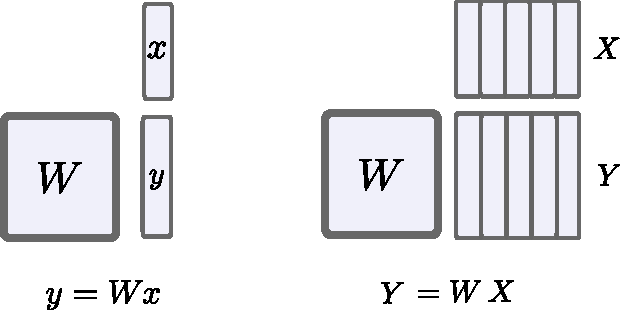
\includegraphics[width=0.80\linewidth]{./figures/batch.pdf}
\end{figure}
$W \in \mathbb{R}^{d_\text{out} \times d_\text{in}}$, $y \in \mathbb{R}^{d_\text{out}}$ and $x \in \mathbb{R}^{d_\text{in}}$ \textbf{VS.}  $Y \in \mathbb{R}^{d_\text{out} \times N}$ and $X \in \mathbb{R}^{d_\text{in} \times N}$
\begin{itemize}
\item Computing linear transformation of \textbf{multiple examples} can be packed into a \textbf{single} matrix-matrix multiplication.
\item Benefit from efficient parallel computation (especially on GPUs).
\item Should write \textbf{vectorized code} instead of loop (example later)
\end{itemize}
\end{frame}


\begin{frame}{Training: Optimization/Optimizer}
\begin{itemize}
\item The parameter update equation in the previous slide:\\
$\theta(n+1) = \theta(n) - \alpha * \nabla_{\theta} \mathcal{L}(\theta(n))$\\
with gradients computed on a mini-batch corresponds to \emphbf{stochastic gradient descent (SGD)} algorithm.
\pause
\item[-] This makes use of the same learning rate $\alpha$ for all parameters.
\begin{itemize}
\item[-] Many other variants for optimization algorithm with adaptive learning rates for each parameter has been proposed.
Popular overview: \link{https://ruder.io/optimizing-gradient-descent/}
\end{itemize}
\pause
\item[-] \textit{adaptive}: change the effective learning rate depending on the past gradients of the corresponding parameter.
\begin{itemize}
\item[-] In particular, \textit{Adam} \citem{kingma15} is very popular.
\end{itemize}
\pause
\item \textbf{Choosing an optimizer = specifying the choice of optimization algorithm and its hyper-parameters.}
\item[-] Hands-on experience in exercises.
\end{itemize}
\end{frame}


\begin{frame}{Some Training Jargon}
\textbf{Progress of training} is often discribed in terms of number of:
\vsp
\begin{itemize}
\item \emphbf{Epochs}: 1 epoch = one run over the whole training data.
\item \emphbf{Steps}: 1 step = 1 gradient update (typically using 1 mini-batch).
\item \emphbf{Updates}: normally synonym to steps.
\item More rarely, \emphbf{sub-epochs}: some fixed fraction of epoch,\\ e.g. 1/4 of epoch.
\end{itemize}
\vsp
The descriptions above are typically correct.\\
But unconventional definitions can also be found in some papers...
\end{frame}

\begin{frame}{Hyper-Parameter Tuning}
 Models have \emphbf{hyper-parameters} such as:
 \begin{itemize}
 \item[-] Number of layers, size of each hidden layer, other model specific hyper-parameters...
 \end{itemize}
\pause
\vsp
So do training algorithms:
 \begin{itemize}
 \item[-] Learning rate, batch size, other optimizer specific hyper-parameters...
 \end{itemize}
\pause
\vsp
Hyper-parameters are not \textit{learned} by the training algorithm!
 \begin{itemize}
% \item They are set before training and remain the same throughout training (with a few exceptions).
 \item \textbf{Tuning}: specify a set of hyper-parameters, train the model, and check its performance on validation data, repeat until you obtain a "good" model.
\item Important, because: \emphbf{model performance can highly depend on the hyper-parameter tuning!}
 \item Tuning is a practice you learn from hands-on experience.
% \item We will come back to this in exercises.
 \end{itemize}

%\begin{itemize}
%\item Both \textbf{model} and \textbf{training algorithm} have hyper-parameters.
%\item They can be \textit{tuned} by looking at model performance on \textbf{validation/development set}.
%\item Important, because: model performance \alertbf{highly depends on the hyper-parameter tuning!}\\
%\item Need to learn to make things to work!
%\end{itemize}
%\vsp
%Illustrated in the exercises.
\end{frame}

\begin{frame}{Summary}
\textbf{What have we learned?}
\begin{itemize}
\item Overview of workflow: main concepts, key words.
\begin{itemize}
\item task \& data, nature of the problem, statistics.
\item evaluation measure
\item model
\item training
\item loss function
\item stochastic gradient descent
\item hyper-parameter tuning
\end{itemize}
\end{itemize}
\vsp
\textbf{Coming up next...}
\begin{itemize}
\item How can we implement these concepts concretely?
\item Introduction to tools for that.
\item ...
\end{itemize}
\end{frame}
